\documentclass[preprint]{acm_proc_article-sp}
%\documentclass[preprint]{sig-alternate}
\usepackage{url}
\usepackage{graphicx,subfigure}
\usepackage{xspace}

\newcommand{\ie}{{\em i.e.,}~}
\newcommand{\eg}{{\em e.g.,}~}

\newenvironment{denseitemize}{
\begin{itemize}[topsep=2pt, partopsep=0pt, leftmargin=1.5em]
  \setlength{\itemsep}{4pt}
  \setlength{\parskip}{0pt}
  \setlength{\parsep}{0pt}
}{\end{itemize}}

\newcommand{\eat}[1]{}


\begin{document}

\title{Project Report: \\
Detecting Spam on Social Networking Sites}

\numberofauthors{3}
\author{
Antonio Lupher,
Cliff Engle,
Reynold Xin\\\\
\texttt{\{alupher, cengle, rxin\}@cs.berkeley.edu}
}

\maketitle

\section{Introduction}
% Modified from project proposal

\subsection{Problem}
Social networks of any significant size see constant spam, scams
and phishing attacks. The nature of these attacks can be quite diverse
and difficult detect. Marketers can spam members with unwanted
advertisements, fraudsters lure users with advance fee frauds and
other confidence tricks, while others attempt to steal user
information by directing users to external phishing pages. To make
matters more difficult, a site with global reach sees communication
among its members in a number foreign languages with varying levels
of ability. This means that much benign content shares characteristics
like misspellings, awkward phrases, etc. that might have made certain
types of common frauds and spam more easy to distinguish on US-based
(or English-language) sites.
% focus on extra impact of non-public features vs. public (bag-of-words)

\subsection{Approach}

This paper examines in detail the types of malicious and benign
content that are encountered on social networks by analyzing
experimental data available from InterPals, an international social network
for cultural exchange and language practice. For example, the site
attracts a wide variety of financial scams, ranging from Nigerian
"419" scams to romance scams. Another prevalent problem is spam with
links to third-party websites, directing users to various porn/webcam
sites, phishing sites or various untrustworthy online marketplaces.

We examine various methods of detecting and preventing abuse
on the site, including those measures that have already been taken
(e.g. various heuristics including IP/location anomaly detection,
frequency capping, duplicate account detection, etc.). We then analyze 
message and user account data points to try to differentiate legitimate users
from malicious ones. By mining this data, we extract features 
to build and evaluate classifiers that can detect unwanted behavior 
programmatically. The large volume of data available to us, although we do 
not use all of it, provides a unique perspective both on the types of
malicious content that exist on such sites as well as on the
effectiveness of classifier-based approaches to identifying
these activities.

We investigated several machine learning techniques to automatically 
detect spam and scams in the private message data, and chose to use 
train and evaluate Naive Bayes, Linear Regression, and 
Support Vector Machine (SVM) classifiers. Our implementations used 
a variety of tools, including Matlab, ScalaNLP, LIBSVM, Lucene and Spark, 
an in-memory distributed computing framework designed for machine 
learning and iterative computation.


\subsection{Data sets}

We enjoyed unrestricted access to the data of InterPals.net, a SNS with 
over 1.3 million active members. This data includes a corpus of over a 
100 million private messages and another 2 million messages that have been 
labeled as spam by users. Other data includes 40 million or so "wall" 
comments, 5 million photos, and 8 million photo comments. 


\section{Background} 

The rapid growth of social media has made Social Networking Services (SNSs) increasingly attractive targets for spam and fraud, leading to a proliferation of sophisticated attacks. This trend is reflected in recent research, as papers have focused on identifying and classifying the various types of social media spam. Many of these studies employ techniques previously used to combat conventional email and web spam. SNSs also provide opportunities to take advantage of user reputation and other social graph-dependent features to improve classification. Nevertheless, most research has been carried out on publicly-available data from SNSs, making it difficult up until now to measure the effect of private user data on algorithms for detecting site misuse.


\subsection{Social Spam Features}

Heymann et al. \cite{heymann} survey the field of spam on SNSs, identifying several common approaches. Identification-based approaches identify spam to train classifiers based on labels submitted by users or trusted moderators. Rank-based approaches demote visibility of questionable content, while interface-based approaches apply policies to prevent unwanted behavior. This work groups classification-based approaches with detection, although classifiers can be used in conjuction with user information to prevent spam before it happens.

A number of researchers have focused on collecting, identifying features and classifying various genres of spam on social networks. Zinman and Donath \cite{zinman} extract bundles of profile-based and comment-based features from MySpace profiles, but the relatively poor performance of their classifier highlights the difficulties in manual classification social network spam. Several studies take the approach of baiting spammers with social ``honeypots", profiles created with the sole intent of attracting spam.\cite{stringhini, lee} They then use the data collected to train classifiers with features including friend request rate and ratios of URLs to text. Webb et al. \cite{webb} use the honeypot approach as well and provide examples of various types of spammers, the typical demographics of their profiles as well as the web pages that they tend to advertise. 

Gao et al. \cite{gao} look at Facebook wall posts, analyzing temporal properties, URL characteristics, post ratios and other features of malicious accounts. They also pinpoint various spam ``campaigns" based on products advertised in a given time frame. They note that spam on Facebook often exhibits burstiness and is mainly sent from compromised accounts. Benevenuto et al. \cite{benevenuto} identify attributes of spam on video SNSs and use a Support Vector Machine (SVM) for classification.

Not all undesirable content on SNSs is necessarily spam or a scam. SNSs and online communities witness inappropriate user behavior, where users post offensive and harassing content. Yin et al. \cite{yin} combine sentiment analysis and profanity word lists with contextual features to identify harassment on datasets from Slashdot and MySpace. Other work looks at SNSs as platforms to collect data about users in order to aid direct attacks on the user's computers or to compromise a large number of accounts. \cite{patsakis, huber}

\subsection{Social Spam Detection Systems}

SocialSpamGuard \cite{jin} is a social media spam detection system that analyzes text and image features of social media posts. The demo system uses GAD clustering \cite{jingad} for sampling spam and ham posts, then trains a classifier with text and image features. However, the system is built on top of Facebook features that are publicly accessible and thus cannot make use of sensitive user data (\eg IP addresses) to increase its effectiveness. 

De Wang et al. \cite{wang} propose a cross-site spam detection framework to share spam data across all social networking sites, building classifiers to identify spam in profiles, messages and web pages. This multi-pronged approach lends itself to associative classification, in which, for example, a message would be classified as spam if it contained a link to a web page that had a high probability of being spam. Unfortunately, the differing characterestics of various social networks \eg the length of messages in Facebook vs. Twitter, can reduce the benefits of sharing spam corpora across diverse sites.

Facebook \cite{stein} provides an overview of their ``immune system" defences against phishing, fraud and spam. The system is composed of classifier services, an ML-derived Feature Extraction Language (FXL), feature loops to aggregate and prepare features for classification and a policy engine to take action on suspected misuse. While the discussion remains high-level and includes few implemention particulars, it does include significant detail on the various types and characterists of undesirable activity on the site, including fake profiles, harassment, compromised accounts, malware and spam. 

In contrast to research that focuses on dynamically detecting spam based on user activity, Irani et al. \cite{irani} show that static features associated with user signups on MySpace are enough to train an effective social spam classifier. They note that C4.5 decision tree algorithms provide better performance than naive Bayes in this case. As in other works, this only examines publicly available profile information collected by social honeypots. Private data collected on users including browser features, IP addresses and geographic location would conceivably improve classifier performance substantially.

Bosma et al. \cite{bosma} explore user-generated spam reports as a tool for building an unsupervised spam detection framework for SNSs. Their approach counts the number of spam reports against a suspected spammer and adds weight to reports based on user reputation. Determining reputation and trustworthiness of users in social networks has been well studied \cite{bian, guha, zhang} and appears to be a promising addition to social spam classification. The framework uses a Bayesian classifier and links messages with similar content, but does not take into account other features. Nevertheless, this is one of the few studies to test its framework on non-public data, inlcuding private messages, spam reports and user profiles from a large Dutch social networking site.

\subsection{Spam Email \& Web}

Much work has been done on protecting traditional email systems from spam. Blanzieri \cite{blanzieri} offers a comprehensive overview of machine learning techniques that can be applied to email filtering. Hao et al. \cite{hao} describe a reputation engine based on lightweight features such as geographic distance between sender and receiver, geolocation anomalies and diurnal patterns. While the target was conventional spam, these and similar features are applicable to spam on SNSs as well.

Whittaker et al. \cite{whittaker} describe a scalable phishing machine learning classifier and blacklisting system with high accuracy. Since a considerable amount of social media spam includes links to phishing sites, being able to detect them is critical. Along similar lines, Monarch \cite{thomas} is a system that provides scalable real-time detection of URLs that point to spam web pages as determined by URL features, page content and hosting properties of the target domain.

Blog comment spam have also attracted considerable attention from researchers who have applied machine learning \cite{kolari, nag} and NLP \cite{mishne} techniques to the problem. Likewise, Markines et al. \cite{markines} apply similar techniques to spam on social bookmarking sites.

\subsection{Machine Learning and Data Mining}

Many of the data mining algorithms used to detect spam and patterns of misuse on SNSs are designed with the assumption that the data and the classifier are independent. However, in the case of spam, fraud and other malicious content, users will often modify their behavior to evade detection, leading to degraded classifier performance and the need to re-train classifiers frequently. Several researchers tackle this adversarial problem. Dalvi et al. \cite{dalvi} offer a modified Naive Bayes classifier to detect and reclassify data taking into account the optimal modification strategy that an adversary could choose. Lowd and Meek \cite{lowd} provide a framework for reverse engineering a classifier to determine whether an adversary can efficiently learn enough about a classifier to effectively defeat it.


\section{Data set}

For this project, we had unlimited access to data from InterPals, a SNS for users who wish to communicate with others from other countries, whether for language practice, cultural exchange or friendship. Users sign up by completing a registration form with information about themselves, including age, sex and location. After registering, users can expand their profile page to include descriptions, interests, languages they speak, etc. and upload photographs. After clicking on a link sent to their email addres, a user can begin to interact with others on the site via private message, public ``wall" posts, comments on photos and on a bulletin board system.

\subsection{Current Anti-Spam Measures}

Currently, the site combats spam and other Terms of Service violations through volunteer moderators. Users can report content, including private messages, profiles and photographs to moderators, using a form that includes a drop-down menu of pre-selected reasons with the option to add a more detailed message in a text field. Likewise, the message interface allows a user to report a private message spam with a single click. Moderators have access to a queue of these reports. In addition to the material being reported, moderators are able to make decisions based on the data from the reported user's account, including outgoing private messages, IP addresses, as well as a list of other users who have logged in from the same computer (determined via IP address as well as by browser fingerprints). Moderators can then decide to delete the user, send a warning, or clear reports on a user. All moderator actions require them to annotate their decision with a brief log message. When deleting a user, moderators have the option of flagging the reported message (if there is one) as spam, or of flagging all of the user's outgoing private messages as spam.

Other anti-spam measures include widespread use of CAPTCHAs across the site and frequency caps. Short-window frequency caps are in place for all users, limiting the number of messages that can be sent per short time interval (1, 5 and 10 minutes). New users are also subject to a per-day cap on the number of unique users with whom they are able to initiate contact. 

Users are able to filter messages by age, sex, continent and country. At this time, 

\subsection{Spam Set}

At the beginning of this research project, there were just over two million messages that had been flagged by moderators as spam. We extracted the contents of exactly two million of these messages from the site's database and merged them with records of account information for the deleted users who had sent the messages. In addition to using SQL to extract much of this information, we wrote Perl scripts to clean the data, tokenize messages and prepare data for further processing. The methodology section (X) offers more details on precisely which items of data were collected and why.

\subsection{Ham Set}

Unlike spam messages, we did not have access to a comparable corpus of human-labeled ham messages. To simplify the labeling of ham messages, we made the assumption that messages remaining in the inboxes of active users after a period of several months would most likely not be spam. Consequently, we extracted a working set of 2 million ham messages that were sent in the beginning of January, 2012 and still existed in the recipient's inbox. To reduce the possibility of collecting messages sent by uncaught spammers to inactive or dormant users, we selected messages only from users and to recipients who had logged in within the last two weeks. As in the case of spam, we collected two million messages with associated account data and merged them into text files for feature extraction.

\subsection{Categories of Spam}

In the course of collecting the data, we observed a number of different types of undesirable messages. Our ongoing observation of spam on the InterPals website provided direct intuition into the major classes of unwanted behavior that we classified as spam for this project. We noted the following broad categories:

\textbf{Advance Fee Fraud} We observed this scam to come in various flavors.  (inheritance, lottery,  etc)
\textbf{Romance Scams:} These 
\textbf{Sexual Solicitation}
\textbf{Porn Ads}
\textbf{Advertising External Sites}
\textbf{Webcam Ads}
\textbf{Money Muling}
\textbf{Begging \& Gift Requests}
\textbf{Business Proposals}


This categorizations are based only on observation. Analyzing the relevant terms in log comments entered by moderators when deleting spammer accounts provides the following breakdown:


\section{Methodology}

We decided to focus on spam in private messages for this paper, given that messages account for a majority of user spam reports. In addition to using the bag-of-words representation of the message content, we aimed to identify a subset of additional, relevant ``expert" features based on public and non-public message and account information that would augment the classifier's accuracy. We first extracted a number of fields that we expected might improve classification. 

To choose a sample of relevant features, we computed statistics on the extracted features, both on the ham and spam corpora. These statistics were generated using SQL on a table created from the merged and cleaned data generated in the process described above. SQL makes it trivial to calculate means and standard errors, but medians are more resource-intensive, so we omitted them from our 

\subsection{Message Features}

\textbf{Message Body \& Subject:} We extracted both the message 

\textbf{Sender IP:} The IP address of the sender at the time that the user sent the message. 

\textbf{Recipient Age/Sex/Country:} These fields were the age, sex and ISO 3166-1 alpha-2 code of the message 
recipient, as listed on their profile. Unfortunately, due to data collection issues, this data was only available 
for the most recent 11,000 spam messages. While the male-to-female ratio of the recipients was very close to that 
of non-spam recipients (both were 47\% male to 53\% female), we found that the age of recipients was typically higher.

\textbf{Recipient Replied:} A boolean, 1 or 0, depending on whether the recipient replied to the message.

\subsection{Sender Account Features}

\textbf{Sender IPs:} Spammers in general had a smaller number of unique IP addresses associated with them than ham users, as per figure \ref{fig:uniqip}. The mean for spammers was 11.82 with a standard deviation of 52.52, whereas ham users saw a mean of 175.51 and standard deviation of 322.19. This is likely due to their comparatively low length of time on the site and the fact that many legitimate users are behind NATs that yield a high number of dynamic IP addresses. One possibility for future research is to investigate the ratio of unique IPs for users as a function of the time they have been registered. Likewise, examining unique /16 network blocks instead of unique IP addresses could mitigate the influence of NATs.

\begin{figure}[h]
    \centering
    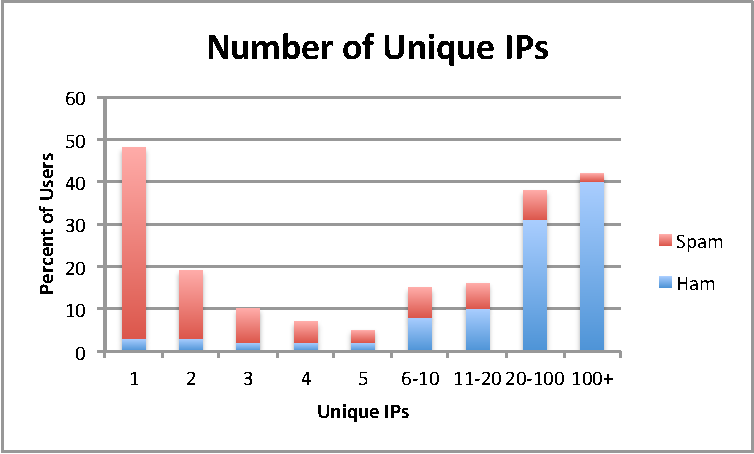
\includegraphics[width=\linewidth]{figures/unique-ips.pdf}
    \caption{Number of unique IP addresses associated with user account. Spam: mean 11.82, std. dev. 52.52. Ham: mean 175.51, std. dev. 322.19}
    \label{fig:uniqip}
\end{figure}

\textbf{Sender Email:} We found that spammers were 

\textbf{Sender Age:} Spam user age 

\textbf{Sender Country:} The distribution of countries as stated by users on their profile and as revealed by their IP address differed remarkably between the spam and ham user groups. 48\% of spam users claimed to be from the United States, with the next most popular countries being UK, Ghana, Senegal, Germany and Canada taking combined 25\%. In contrast, only 15\% ham users claimed to be from the United States, with Russia, Korea, UK, France and Germany combining for 24\%. 

figure \ref{fig:usaspam}
figure \ref{fig:usahamfig:lambda}
\begin{figure}[h]
    \centering
    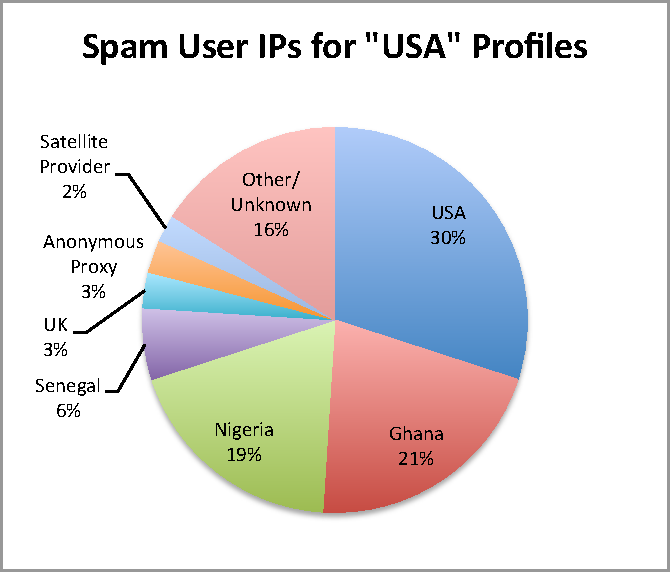
\includegraphics[width=\linewidth]{figures/ips-usa-spam.pdf}
    \caption{Distribution of IPs by country for spammers with profiles stating a USA location.}
    \label{fig:usaspam}
\end{figure}


\begin{figure}[h]
    \centering
    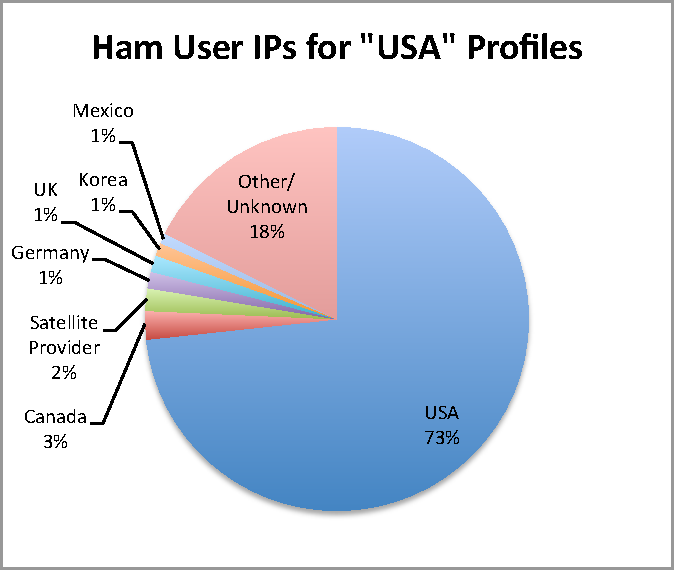
\includegraphics[width=\linewidth]{figures/ips-usa-ham.pdf}
    \caption{Distribution of IPs by country for ham users with profiles stating a USA location.}
    \label{fig:usaham}
\end{figure}


\textbf{Sender Birthday:}

We also noticed that Afghanistan and Albania featured prominently at the 11th and 15th most popular countries f......

\textbf{Sender Age:}

\textbf{Sender Name:}



\textbf{Username, Name:} While we collected these fields, we did not end up processing or analyzing them further. That said, we saw considerable repetition in the usernames of scammers and it seems that analyzing the substrings in these fields could yield useful features.

\textbf{Sender Sex:}

\subsection{Mixed Features}

\textbf{Account Lifetime.}

\textbf{IP Mismatch.} This 




\section{Classification}

\subsection{Naive Bayes}

% Modified from Reynold's HW1  write-up
%We use a na\"ive Bayes model, in which the documents are generated according to the following process.  
%First, a class \(c\) is chosen from a probability distribution \(\Pr(c)\).
%Then, a document from class \(c\) is generated.
%We tried a multinomial model and a Bernoulli model to model this process.
%\begin{itemize}
%\item \emph{Multinomial model.}  A document length \(m_d\) is chosen and \(m_d\) words \(w_{d,1}, \dotsc, w_{d,m_d}\) are chosen independently from a distribution \(\Pr(w|c)\).
%\item \emph{Bernoulli model.}  For each word \(w\) in the vocabulary, \(w\) is added to the document with probability \(\Pr(w|c)\).
%\end{itemize}
%The distributions \(\Pr(c)\) and \(\Pr(w|c)\) are parameters of the model.
%
%
\subsection{Linear Regression}

% Modified from Cliff & Antonio's HW2 write-up
%Linear regression is a method to model the relationship between an output variable, $y$, and explanatory variables, $X$. The output variable is a linear sum of the explanatory variables multiplied by their corresponding coeffecients, represented by $\beta$. In our case, $y$ represents a review's ranking from one to five, while $X$ is the bag-of-words representation of the review text. This implies that $\beta$ represents the weight of a word's correlation to a higher review. This gives us the simple regression formula: $$y=X\beta$$
%
%In this project, we performed ordinary least squares regression. By minimizing the sum of squared residuals, we can solve for the unkown parameter vector $\beta$ using a closed form solution. $$\beta=(X'X)^{-1}X'y$$ In order to ensure that the matrix $X'X$ is invertible, we perform ridge regression. In ridge regression, we add the identity matrix, $I$, scaled by a factor, $\lambda$, to produce the following equation. $$\beta=(X'X+\lambda I)^{-1}X'y$$ We calculate this $\beta$ for a training set of review text along with their corresponding ratings which range from 1 to 5. We then evaluate our model $\beta$ on the withheld reviews in order to perform a 10-fold cross-validation.
%
%All of our linear regression code was implemented in MATLAB because of its ease-of-use and optimizations on matrix multiplications. We parsed the reviews from the tokenized binary format into a bag-of-words representation stored as a sparse matrix. Matlab uses Compressed Sparse Column format, so we actually stored the matrix $X'$ because the dictionary is very sparse. We also filtered out duplicate reviews by hashing the first ten words in a review to determine distinctness. This filtered the one million reviews to 492,130. 
%
%The actual matrix multiplications were done using the sparse $X$ matrix along with our $y$ vector and the ridge parameter. The multiplication $X'X$ takes up too much memory if we use the entire dictionary, so we chose to limit the dictionary size. We found that a dictionary of the 10,000 most frequent words gave sufficient features while also being computable using MATLAB's built-in sparse matrix multiplications. We also tried using a dictionary of 15,000 words, but only had a marginal improvement along with much slower execution. Using our 10,000 word dictionary, we calculated the performance of our matrix multiply to be 0.123 Gflops/s by dividing the number of non-zero elements in our matrices by the time to compute the multiplication. 
%
%
%Since we used ridge regression, we had the ability to tune the $\lambda$ parameter in order to get the best performance. As shown in figure \ref{fig:lambda}, we observed an AUC improvement of about .5\% between the default value of 1 and a tuned parameter of 1500. This is a fairly major difference since the AUC is at 93\% using the default value. Additionally, we also noticed a major difference in the top words when using better $\lambda$ values. Using the default value of 1, our top words included obscure words including ``\_c'', ``\_j'', ``donovan'', and ``matlock.'' When we used the tuned $\lambda$ value of 1500, the words were much more representative, as shown in table \ref{tab:words}.
%




\subsection{Logistic Regression}

We attempted to train the multiple logistic regression classifier implemented by the ScalaNLP package, but encountered a bug that prevented the model from being generated correctly. With the expectation that SVMs would outperform logistic regression, we decided to focus our efforts on tuning the SVM instead of pursuing logistic regression. 


\subsection{Support Vector Machines (SVMs)}

%intro to svms

Support Vector Machines are a classification method  \cite{boser}, \cite{cortesv95} 

% scalanlp svm 

% libsvm

LIBSVM is library for SVM training and classification in C++ and Java, with wrappers for Python and other languages. The package allows one to specify the type of kernel to use, kernel parameters ($\gamma$, $\rho$, $d$), as well as a penalty parameter ($C$). We used Perl to convert the sparse feature matrices generated for use with ScalaNLP to a format recognized by LIBSVM. We then used one of the package's tools to perform simple scaling on the data. 

Given the complexity of choosing kernels and parameters, the package includes a Python script that performs cross-validation to suggest appropriate $\gamma$ and $C$ values for the recommended radial basis function (RBF) kernel. The RBF kernel is a real-valued function such that 

\begin{itemize}
\item $K(\mathbf{x}_i, \mathbf{x}_j) = (\gamma\mathbf{x}_i^\intercal\mathbf{x}_j+r)^d, \gamma>0$
\end{itemize}
We ran this script on a subset of 2500 ham and 2500 spam messages to obtain $C = 8$ and $\gamma = 0.0078125$.

The LIBSVM scaling tool increases file size considerably for data sets with large feature matrices. This large file size, coupled with the computational resources required for SVM training on large data sets, prevented us from completing our analysis of the 

%\begin{tabular}{c|c|c}
%    \multicolumn{3}{c}{Unscaled: Data set size, Accuracy (bag-of-words), Accuracy (expert features)}
%    Data size & Accuracy, bag-of-words & Accuracy, expert features \\
%    \hline
%    2k & 0.0 & 0.0 \\
%    10k & 0.0 & 0.0 \\
%    22k & 0.0 & 0.0 \\ % note we chose 22k because 11k had the recipient info
%    50k  & 0.0 & 0.0 \\
%    100k  & 0.0 & 0.0 \\
%\end{tabular}
%
%
%\begin{tabular}{c|c|c}
%    \multicolumn{3}{c}{Scaled: Data set size, Accuracy (bag-of-words), Accuracy (expert features)}
%    Data size & Accuracy, bag-of-words & Accuracy, expert features \\
%    \hline
%    2k & 0.0 & 0.0 \\
%    10k & 0.0 & 0.0 \\
%    22k & 0.0 & 0.0 \\ % note we chose 22k because 11k had the recipient info
%\end{tabular}
%


\section{Results}


\subsection{Linear Regression}

%\begin{tabular}{c|c}
%    \multicolumn{2}{c}{Tokens most likely to be positive} \\
%    token & \(log(p_+ / p_-)\) \\
%    \hline
%    pos & 0.0 \\
%    pos2 & 0.1 \\
%\end{tabular}
%
%\begin{tabular}{c|c}
%    \multicolumn{2}{c}{Tokens most likely to be negative} \\
%    token & \(log(p_+ / p_-)\) \\
%    \hline
%    neg & 0.0 \\
%    neg2 & 0.1 \\
%\end{tabular}
%

\subsection{SVMs}

%\begin{tabular}{c|c}
%    \multicolumn{2}{c}{Tokens most likely to be positive} \\
%    token & \(log(p_+ / p_-)\) \\
%    \hline
%    pos & 0.0 \\
%    pos2 & 0.1 \\
%\end{tabular}
%
%\begin{tabular}{c|c}
%    \multicolumn{2}{c}{Tokens most likely to be negative} \\
%    token & \(log(p_+ / p_-)\) \\
%    \hline
%    neg & 0.0 \\
%    neg2 & 0.1 \\
%\end{tabular}
%

\section{Analysis}
% Vern wants site owner perspective on how to apply classifiers
From a site's perspective, ...

\section{Future Work}

\subsection{Spam Grouping}

As a part of this project, we performed some qualitative analysis on spam and differentiated between the major categories of undesirable messages found on this SNS. However, we 

Characteristics of spam messages vary widely depending on the type of spam
we currently lump all spam into a single category; we plan to build on the classes we mentioned in section()
We are currently in the process of extending the moderation interface to include more specific tagging capabilities
%- certain classifiers might work better on certain types of spam
%- clustering to see how well these classes fit the spam types on the site


\subsection{Features}

In this project, we chose only a small subset of ``expert" features to use. However, we believe that it would be beneficial to train and evaluate the classifiers on a wider range of features. The features would include both the ones we extracted in this project but omitted from the classifier features matrices, as well as new features. Adding N-grams and message similarity tests seem particularly promising. N-grams would allow the classifier to take into account certain phrases \eg{``Western Union" or ``money transfer"}. 

We have also recently begun to collect browser fingerprints from users based on user agent and JavaScript-acquired browser plugin details, time zone, screen size, color depth, system fonts, keyboard layout and locale information. Subsequent classifiers could leverage this information either as a hash that effectively tags individual known spammers or in part, adding features based on time zone or keyboard layout.

It is also anecdotally clear from moderator log messages that spammers re-use their profile photos and these photos are often of celebrities, porn stars or simply stock photos. Hashing these images 


Server access logs, search logs and user viewing histories from InterPals, all of which are available to us, offer another avenue for future research. It is conceivable that certain spammers may have similar site usage patterns, in terms of HTTP request intervals, 


\subsection{Testing \& Evaluation}

- test SVM and other classifiers on newer data
- 

\section{Conclusion}




figure \ref{fig:cprof}
figure \ref{fig:cip}
figure \ref{fig:day}
figure \ref{fig:month}
figure \ref{fig:drop}
figure \ref{fig:email}
figure \ref{fig:friends}
figure \ref{fig:roclin}
figure \ref{fig:photos}
figure \ref{fig:recipage}
figure \ref{fig:sendage}
figure \ref{fig:sendsex}
figure \ref{fig:roc-25}
\begin{figure}[h]
    \centering
    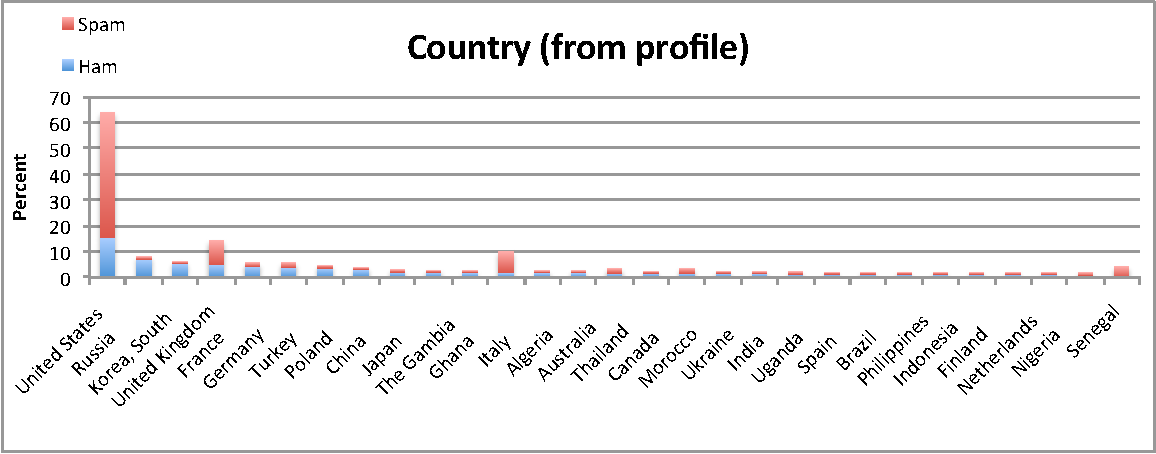
\includegraphics[width=\linewidth]{figures/country-prof.pdf}
    \caption{Country as stated on user profile.}
    \label{fig:cprof}
\end{figure}

\begin{figure}[h]
    \centering
    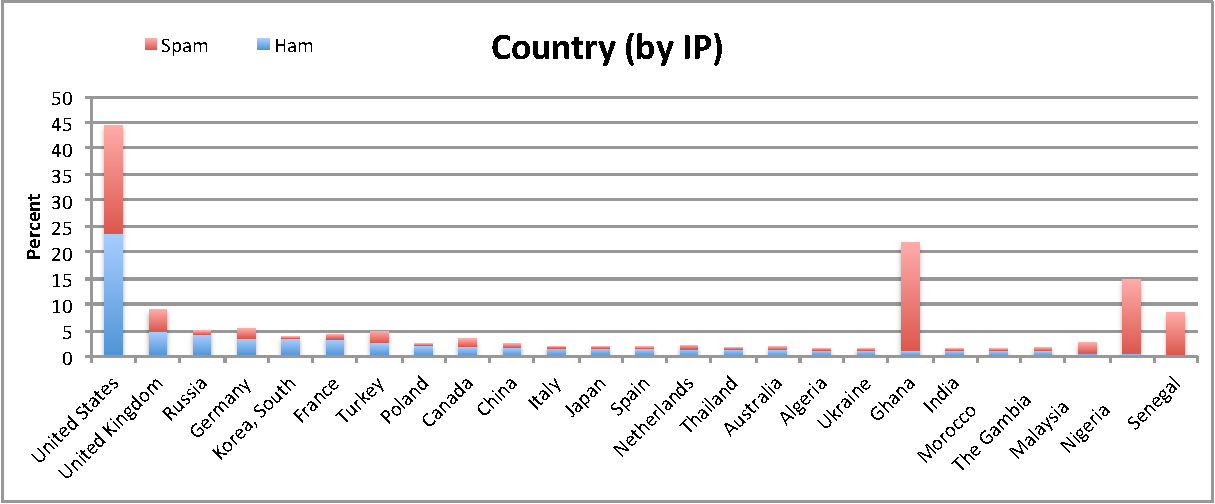
\includegraphics[width=\linewidth]{figures/country-ip.pdf}
    \caption{Country detected by IP address using MaxMind GeoIP database.}
    \label{fig:cip}
\end{figure}

\begin{figure}[h]
    \centering
    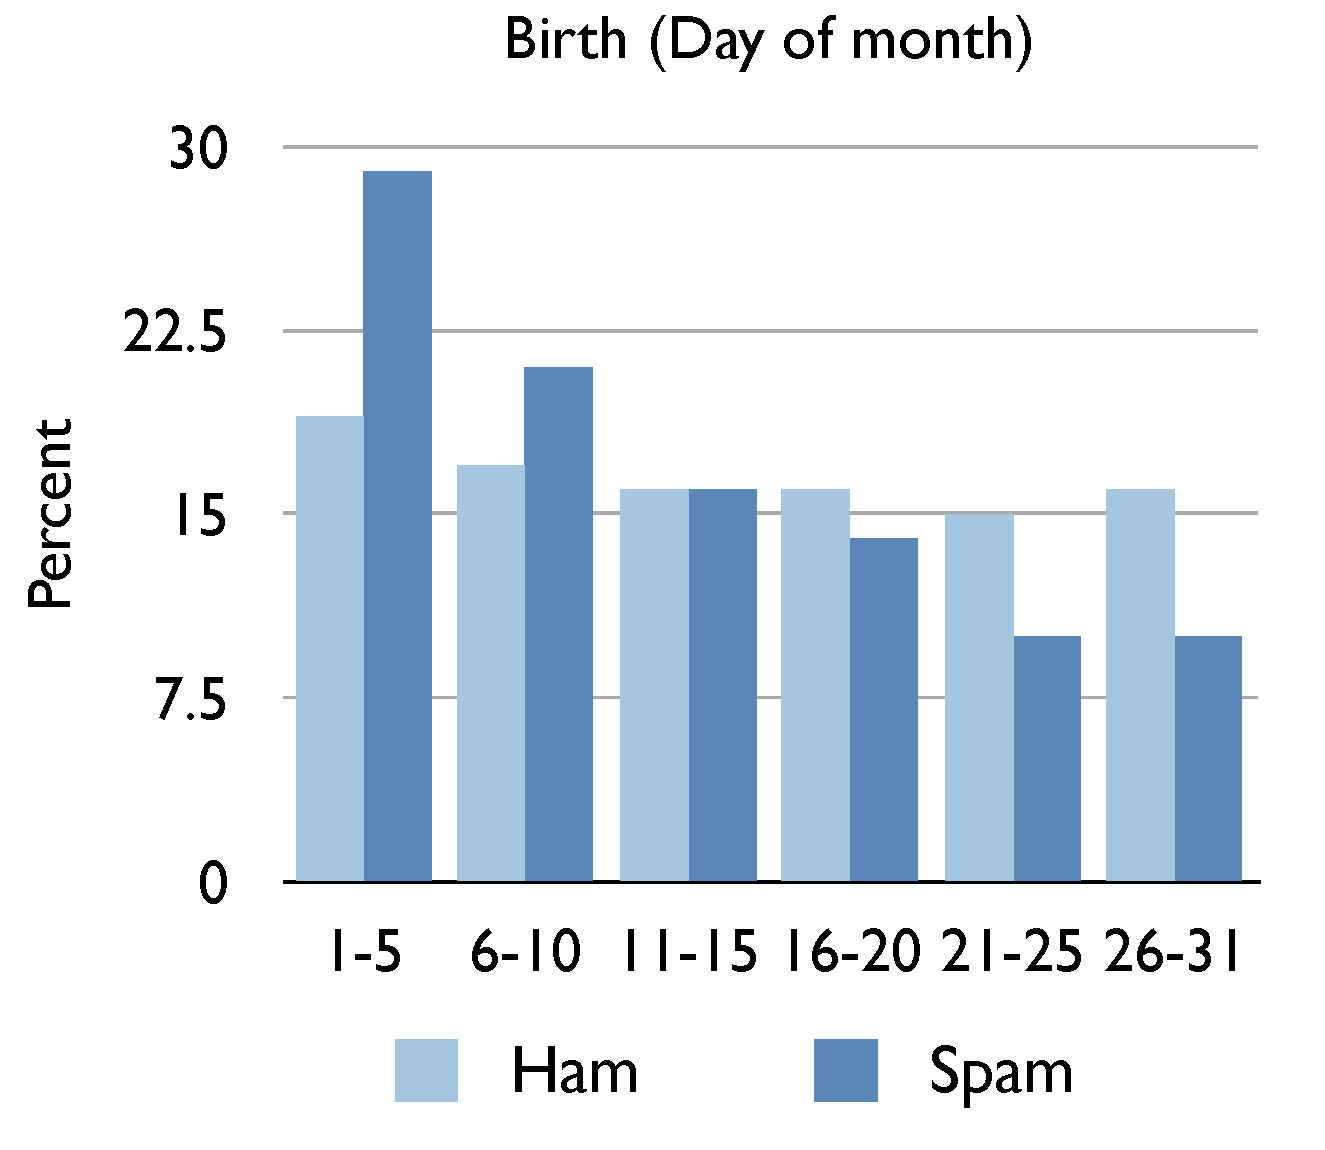
\includegraphics[width=\linewidth]{figures/dob-day.pdf}
    \caption{Date of month from birthday submitted by user at signup.}
    \label{fig:day}
\end{figure}

\begin{figure}[h]
    \centering
    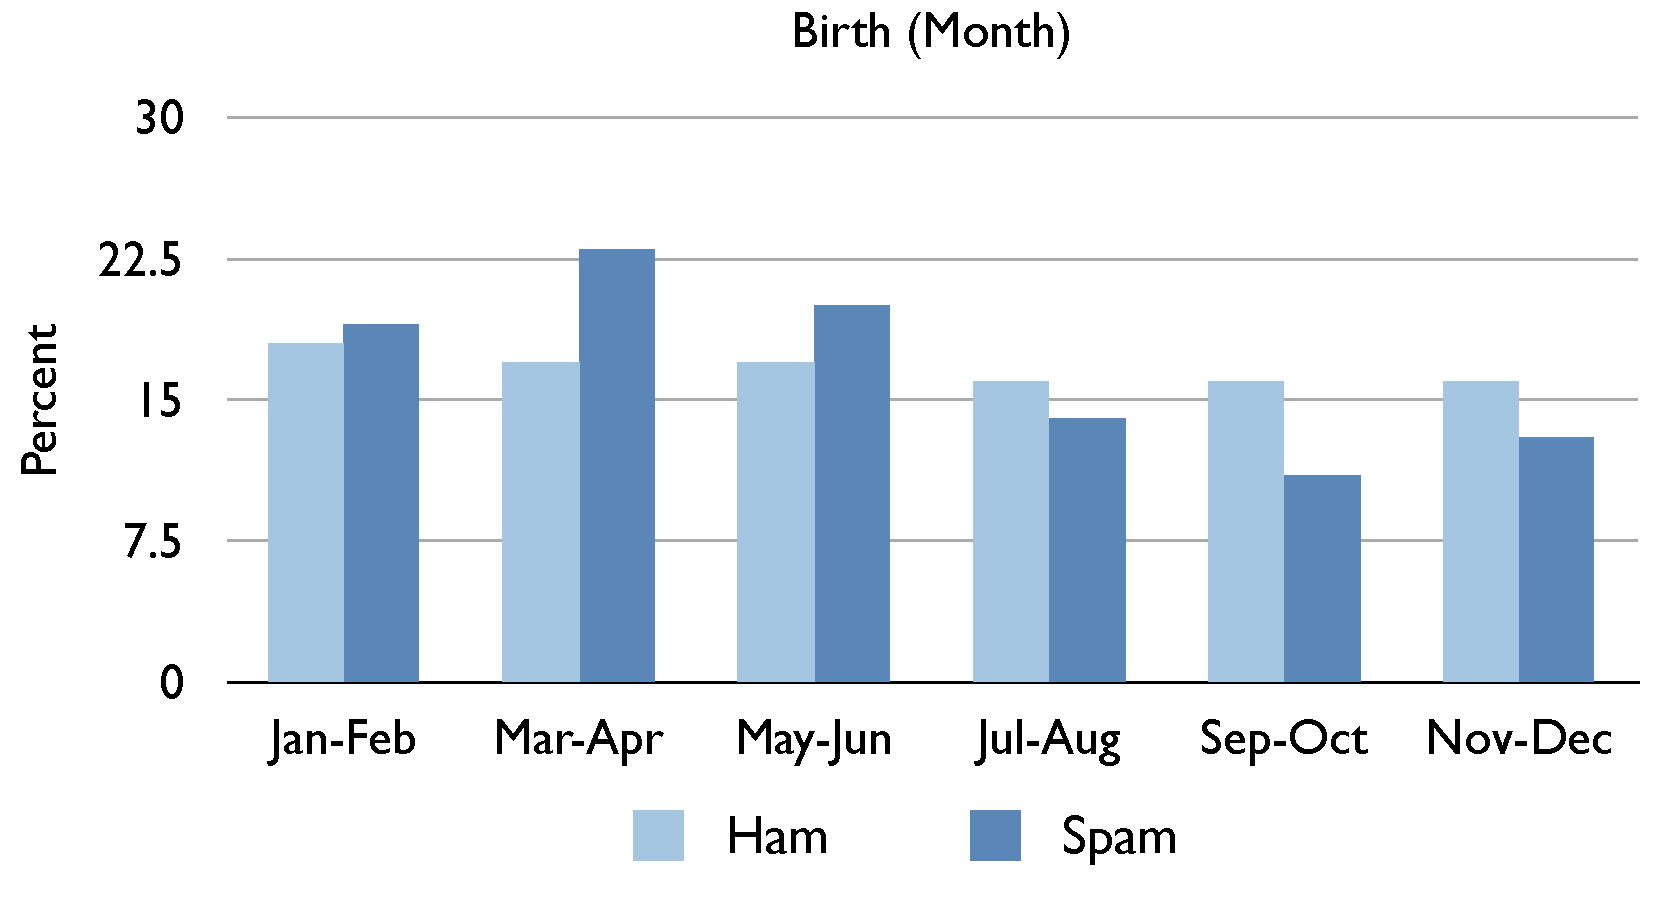
\includegraphics[width=\linewidth]{figures/dob-month.pdf}
    \caption{Month of birthday as submitted by user at signup.}
    \label{fig:month}
\end{figure}

\begin{figure}[h]
    \centering
    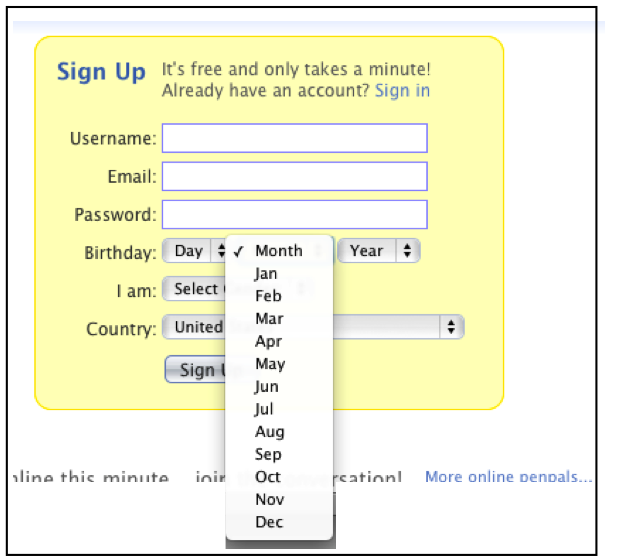
\includegraphics[width=\linewidth]{figures/dropdown.png}
    \caption{Drop-down select menu on signup form.}
    \label{fig:drop}
\end{figure}

\begin{figure}[h]
    \centering
    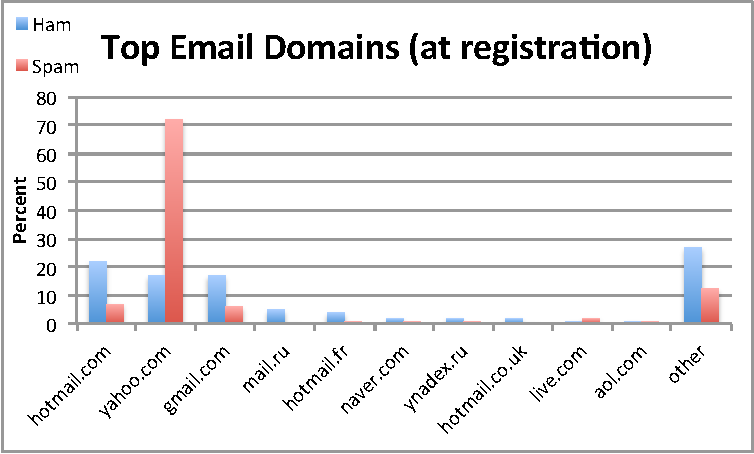
\includegraphics[width=\linewidth]{figures/email.pdf}
    \caption{Domain name of email provided at signup. Users cannot send messages before 
        activating their account via a link sent to their email address.}
    \label{fig:email}
\end{figure}

\begin{figure}[h]
    \centering
    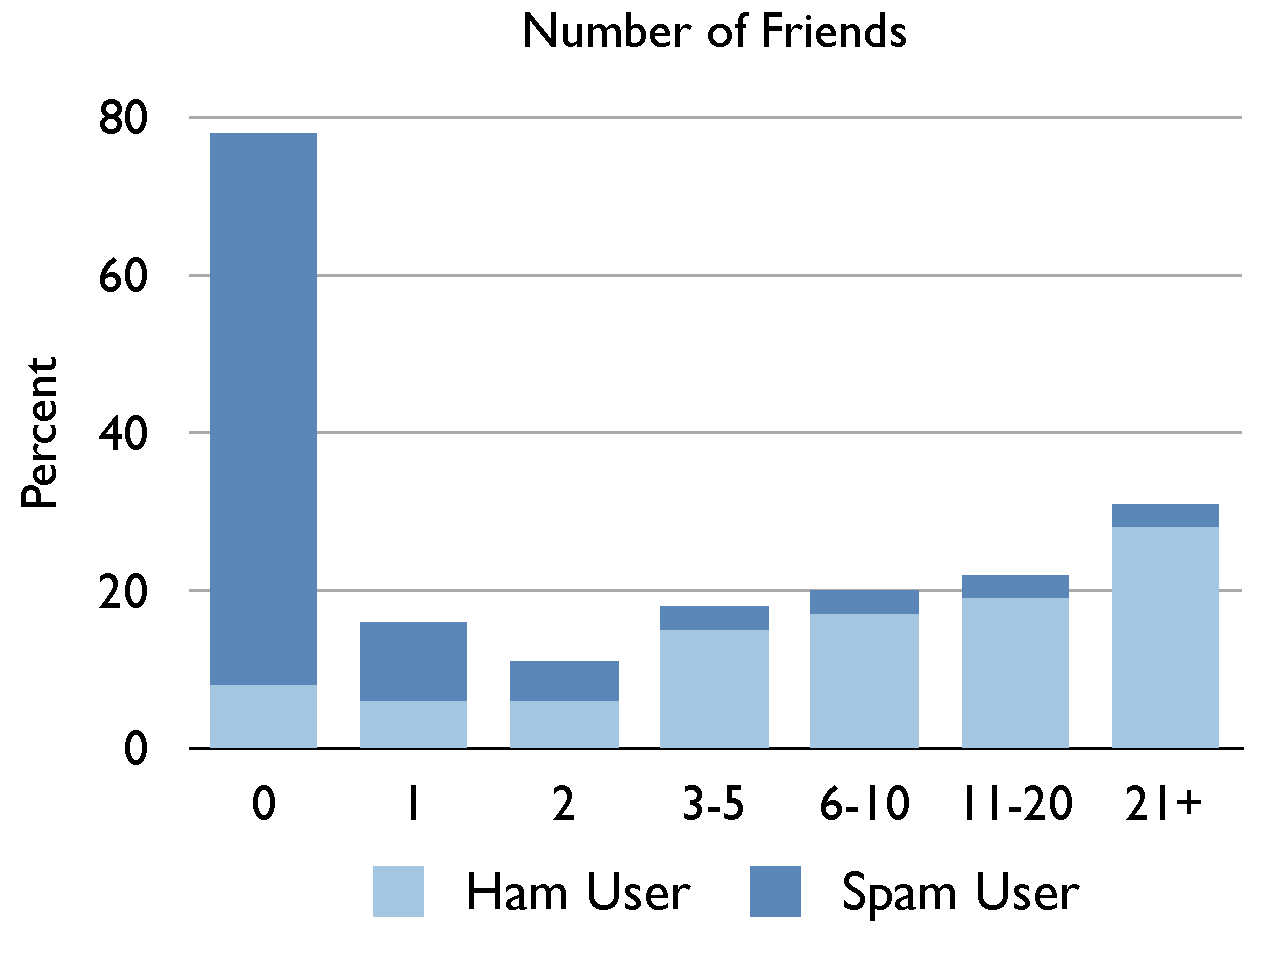
\includegraphics[width=\linewidth]{figures/friends.pdf}
    \caption{Number of friends associated with sender account.}
    \label{fig:friends}
\end{figure}


\begin{figure}[h]
    \centering
    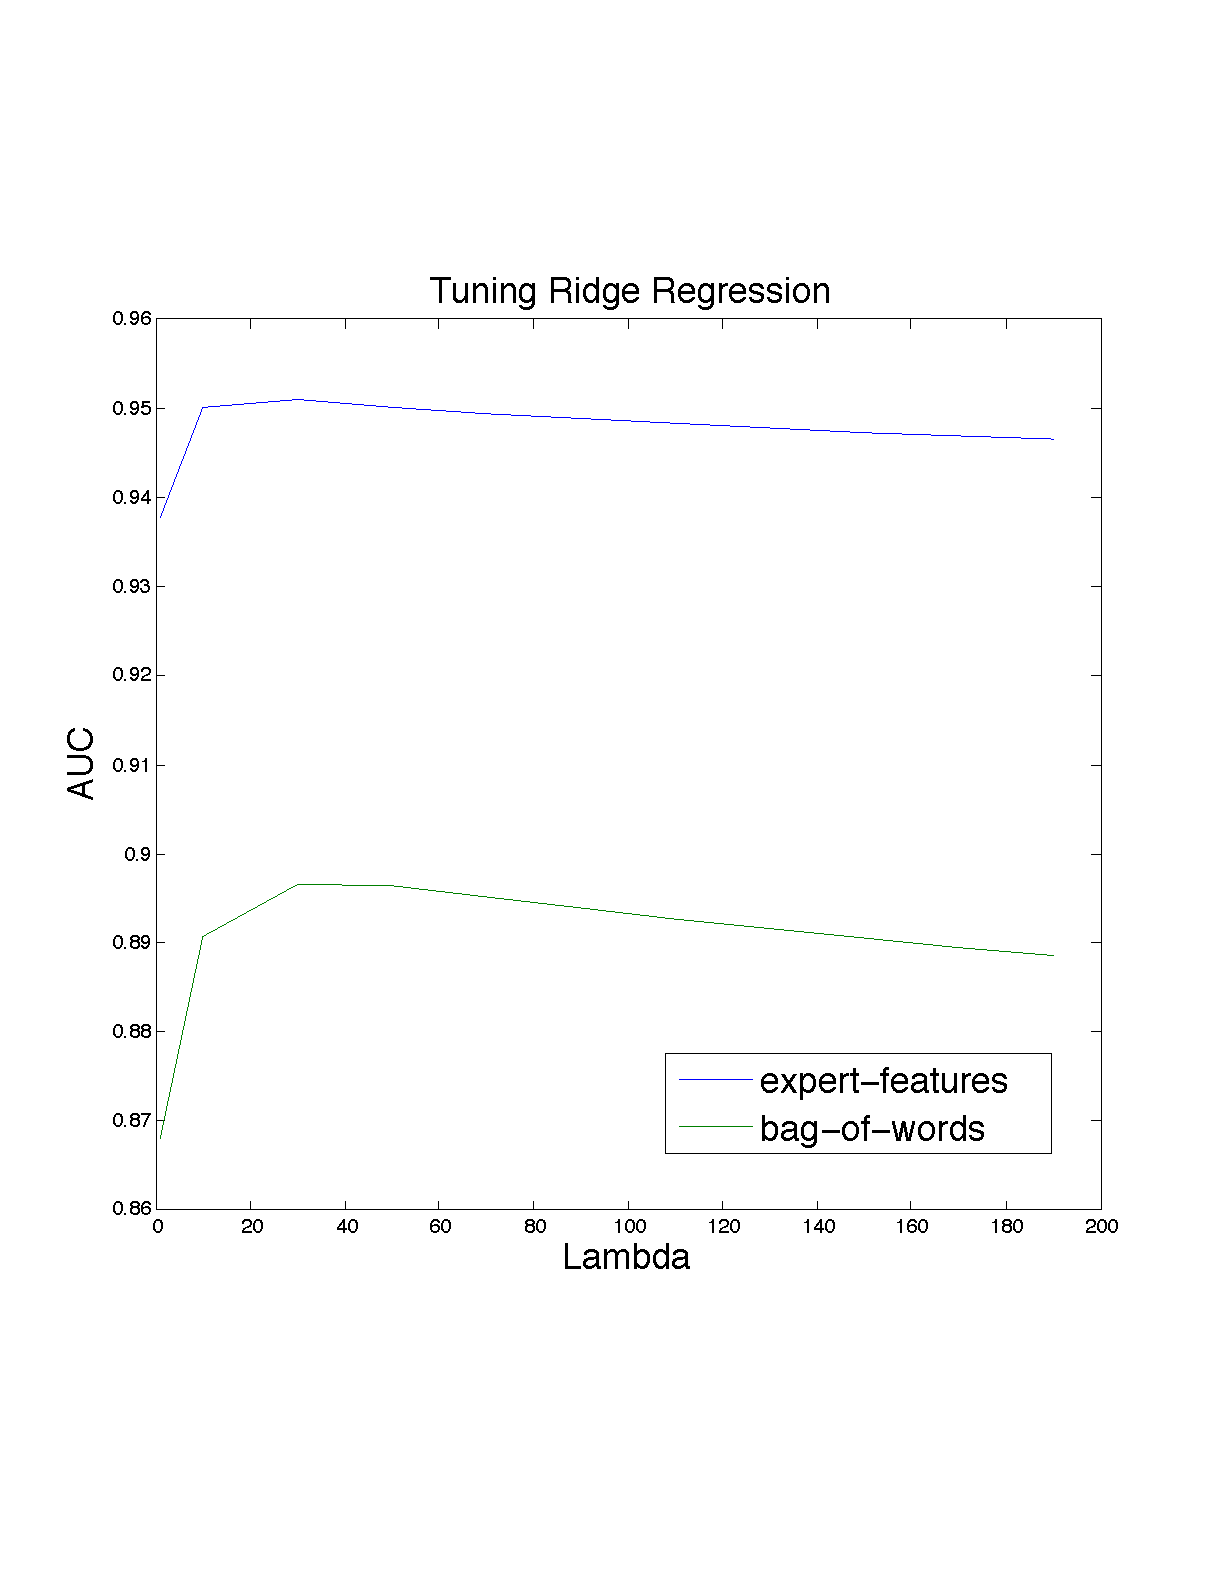
\includegraphics[width=\linewidth]{figures/linear-ridge.pdf}
    \caption{AUC based on varying lambda values for Ridge regression.}
    \label{fig:lambda}
\end{figure}

\begin{figure}[h]
    \centering
    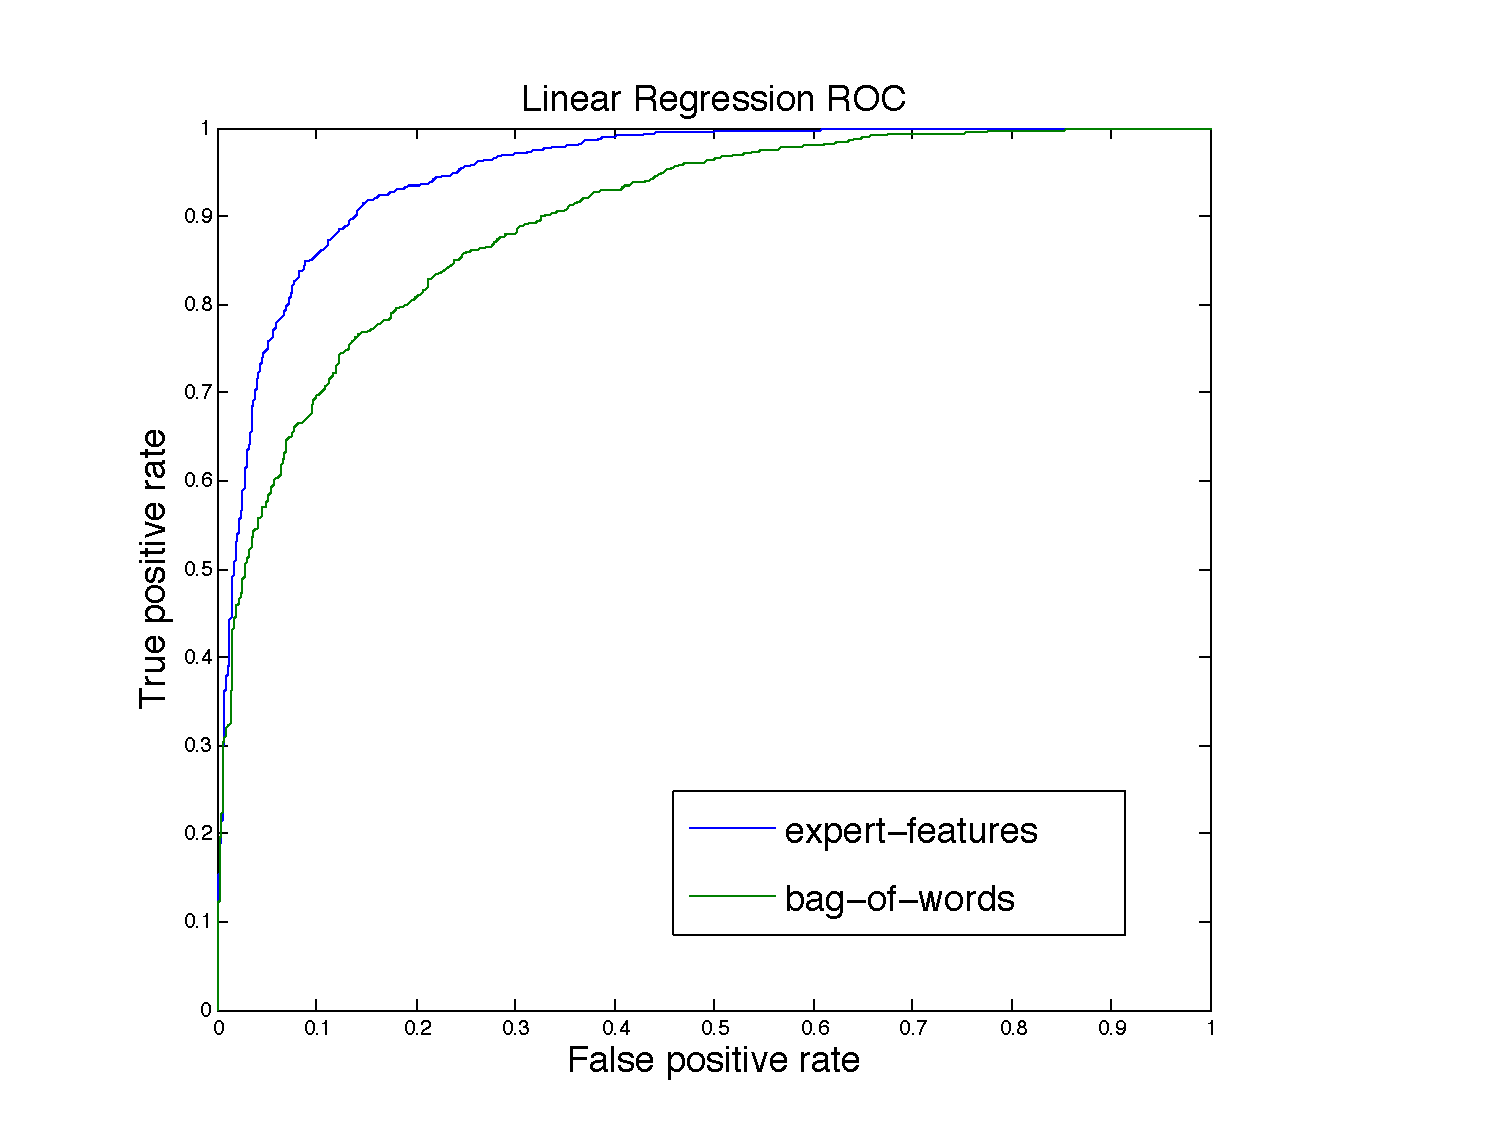
\includegraphics[width=\linewidth]{figures/linear-roc.pdf}
    \caption{Linear regression ROC curves for classifier using bag-of-words and bag-of-words with ``expert" features.}
    \label{fig:roclin}
\end{figure}

\begin{figure}[h]
    \centering
    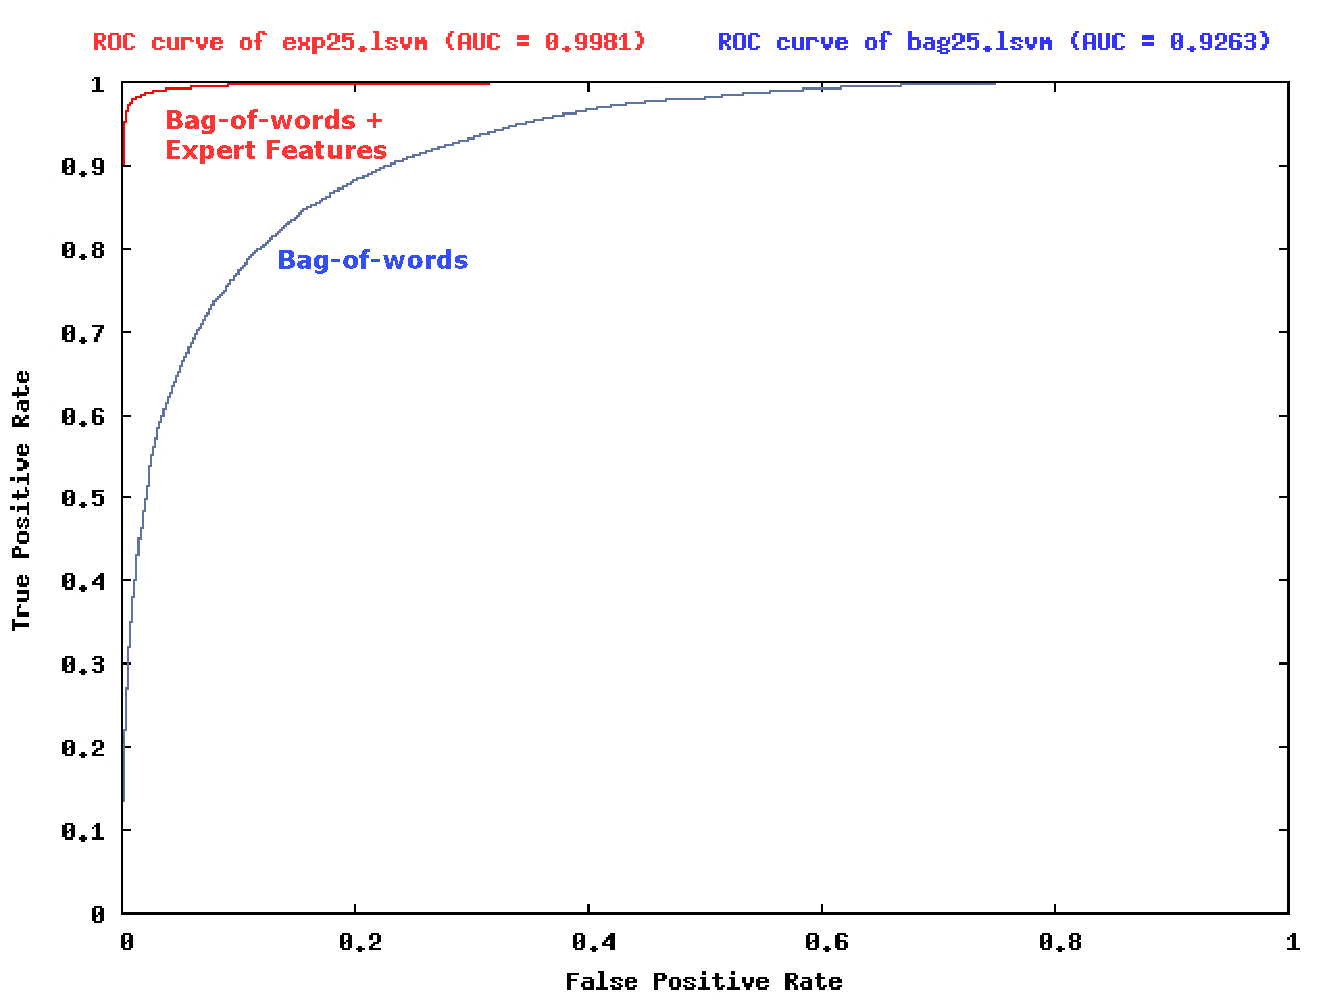
\includegraphics[width=\linewidth]{figures/roc-25.pdf}
    \caption{LIBSVM ROC curves for classifier using bag-of-words and bag-of-words with ``expert" features on 50k messages.}
    \label{fig:roc-25}
\end{figure}


\begin{figure}[h]
    \centering
    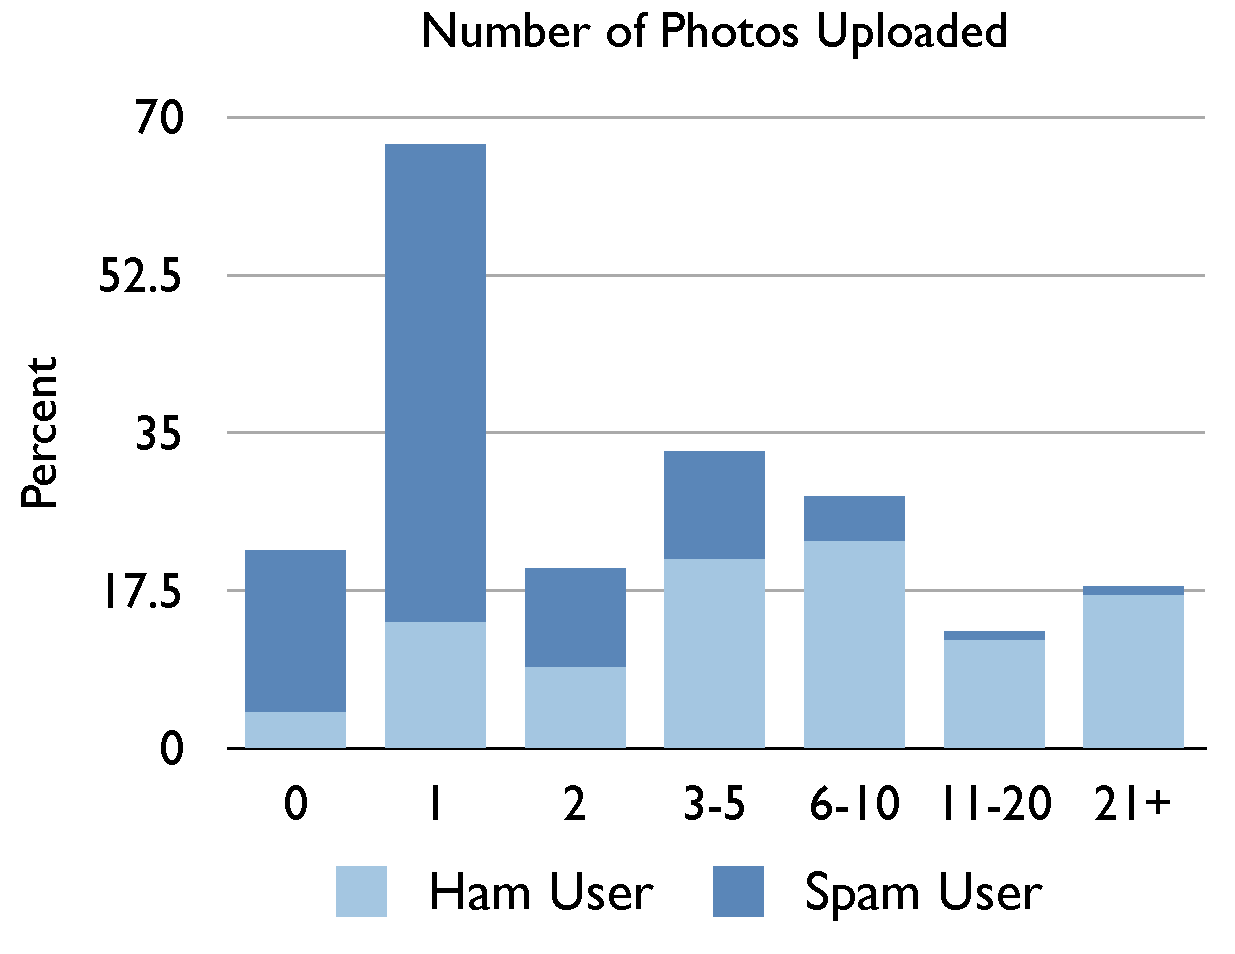
\includegraphics[width=\linewidth]{figures/photos.pdf}
    \caption{Number of photos associated with sender account.}
    \label{fig:photos}
\end{figure}

\begin{figure}[h]
    \centering
    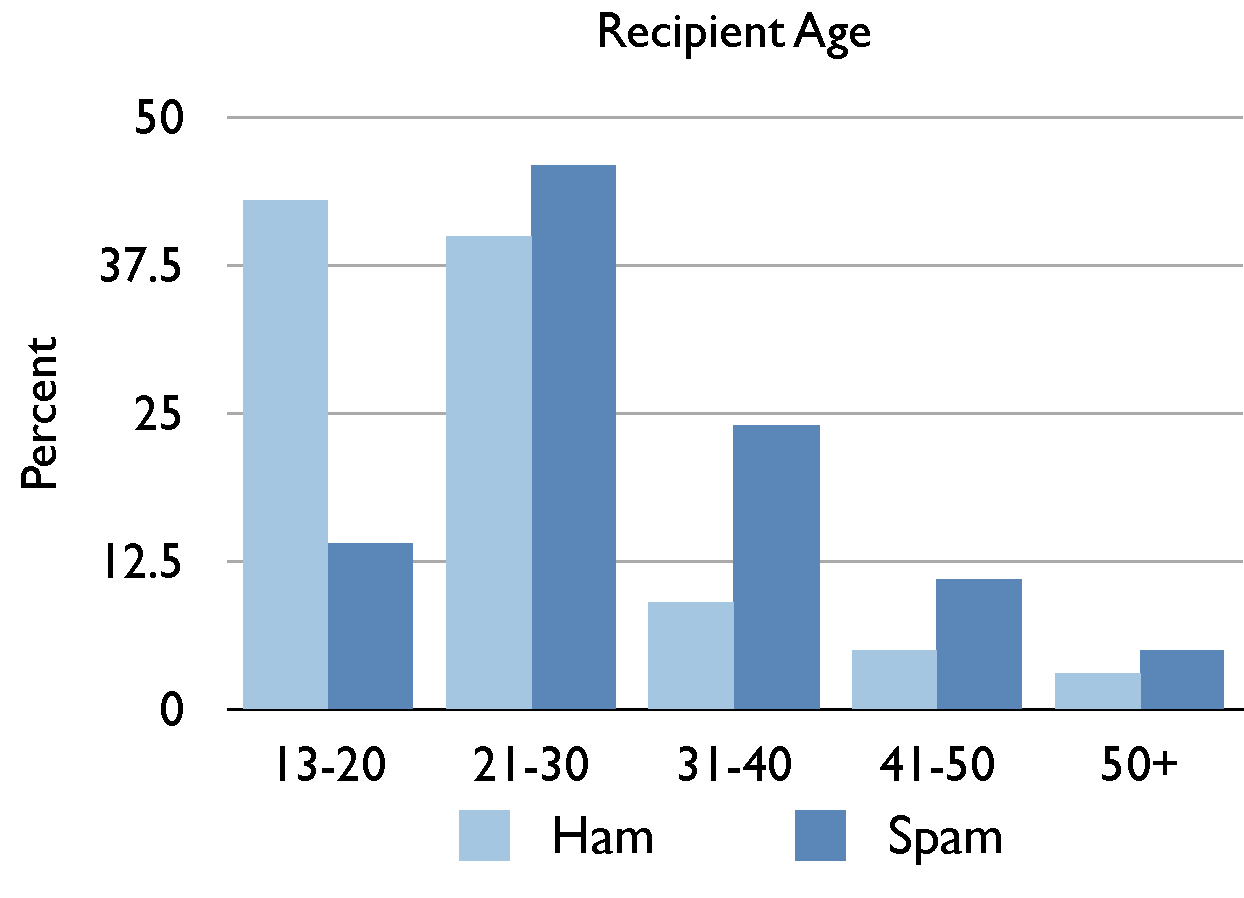
\includegraphics[width=\linewidth]{figures/recip-age.pdf}
    \caption{Age of message recipient as stated on user profile. Note that 2 million message spam sample 
        had only 11,000 messages with this information.}
    \label{fig:recipage}
\end{figure}

\begin{figure}[h]
    \centering
    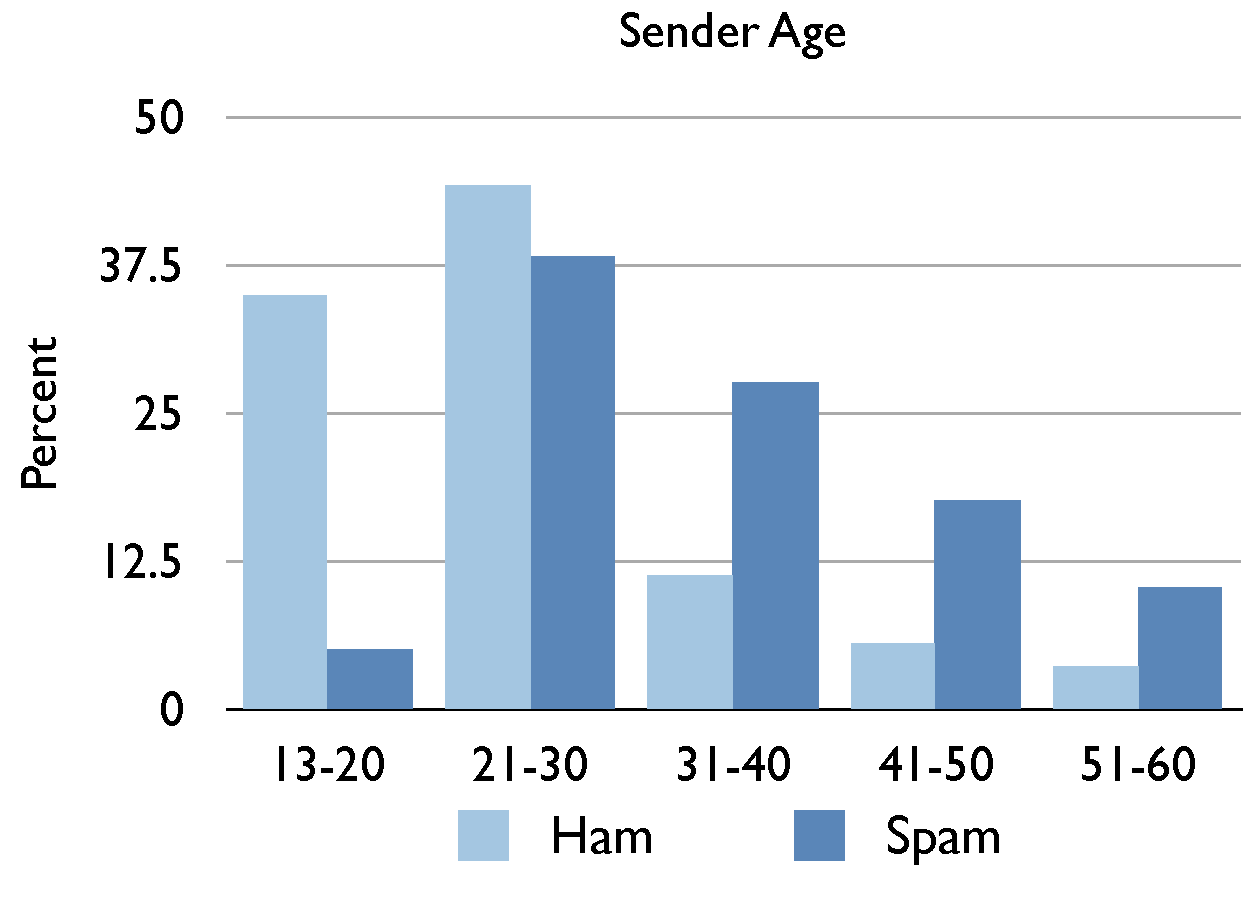
\includegraphics[width=\linewidth]{figures/sender-age.pdf}
    \caption{Age of message sender as stated on user profile. }
    \label{fig:sendage}
\end{figure}

\begin{figure}[h]
    \centering
    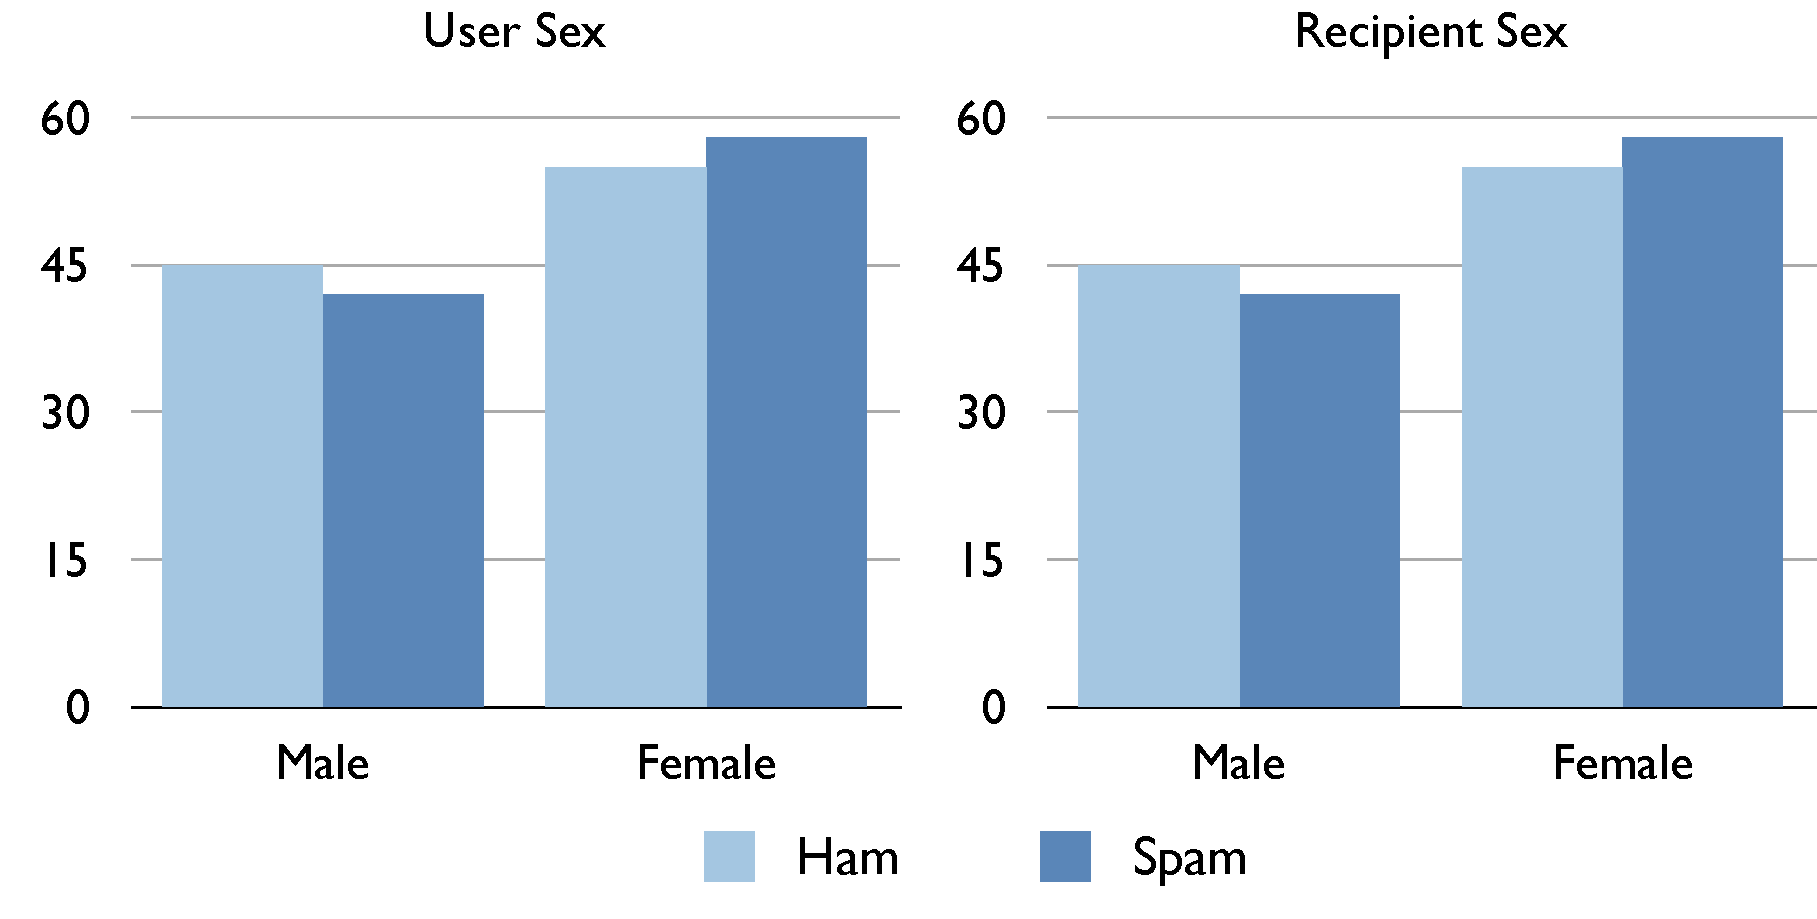
\includegraphics[width=\linewidth]{figures/sex.pdf}
    \caption{Sender sex as stated on profile.}
    \label{fig:sendsex}
\end{figure}




\bibliographystyle{abbrv}
\bibliography{paper}



\balancecolumns
\end{document}
